
\documentclass[serif]{beamer}


\usepackage{txfonts}

\usepackage{verbatim}
\usepackage{amssymb}
% \usepackage{pgf,pgfarrows,pgfautomata,pgfheaps,pgfnodes,pgfshade}
% \usepackage{multimedia}
\usepackage[utf8]{inputenc}
\usepackage[T1]{fontenc} 
\usepackage{aeguill}
\usepackage[french]{babel}
\usepackage{fancybox}
\usepackage{fourier-orns,eurosym,tikz}
\usepackage{soul}
\usepackage{threeparttable}
\usepackage{amssymb}% http://ctan.org/pkg/amssymb
\usepackage{pifont}% http://ctan.org/pkg/pifont
\newcommand{\cmark}{\ding{51}}%
\newcommand{\xmark}{\ding{55}}%

\definecolor{kugreen}{RGB}{50,93,61}
\usetheme{Singapore}%Darmstadt}%nom du theme global
% \usecolortheme[named=kugreen]{structure}%nom du theme de couleur
%\usecolortheme{wolverine}
\usefonttheme{}%nom du theme de police
\useinnertheme{}%nom du theme interne
\useoutertheme{}%nom du theme externe

%\useinnertheme[shadow=true]{rounded}
%\useoutertheme{infolines}
%\usecolortheme{beaver}

\setbeamerfont{block title}{size={}}
\setbeamercolor{titlelike}{parent=structure,bg=white}


\newcommand{\tr}[1]{
	{\color{red}{ #1}}
}
\newcommand{\tb}[1]{
	{\color{blue}{\bf #1}}
}
\definecolor{VertFonce}{rgb}{0,.4,.0}

\newcommand{\trr}[1]{
	{\bf \color{red}{ #1}}
}
\newcommand{\tv}[1]{
	{\color{VertFonce}{\bf #1}}
}
\newcommand{\tvs}[1]{
	{\color{VertFonce}{#1}}
}
\newcommand{\degree}{^{\circ}}

\newcommand{\E}{\mathrm E}
\newcommand{\Var}{\mathrm{Var}}
\newcommand{\Cov}{\mathrm{Cov}}


\newcommand{\bX}{\mathbf{X}}
\newcommand{\bY}{\mathbf{Y}}
\newcommand{\bx}{\mathbf{x}}
\newcommand{\by}{\mathbf{y}}
\newcommand{\bz}{\mathbf{z}}
\newcommand{\bZ}{\mathbf{Z}}
\newcommand{\bbeta}{\boldsymbol{\beta}}

\newcommand{\Cite}[1]{${\scriptsize [\mbox{#1}]}$}
\title[Quantiles and point processes]{Regularization techniques for spatial point processes intensity estimation}

\author{ {Jean-Fran\c{c}ois Coeurjolly \\ 
{\small (joint work with A. Choiruddin, F. Letué) }}
% {\scriptsize\texttt{http://www-ljk.imag.fr/membres/Jean-Francois.Coeurjolly/}}
}

% \institute[LJK]{\vspace*{-.5cm}Laboratoire Jean Kuntzmann (LJK),  Grenoble University  \bigskip
% \institute[LJK]{
% } 
  % \includegraphics[scale=.32]{img/summer2010.pdf} \includegraphics[scale=.35]{img/qk.pdf} 
  % } 

\date{} 
% Fin de la partie titre
%\setbeamertemplate{background canvas}{\includegraphics
%   [width=\paperwidth,height=\paperheight]{fondecran3.pdf}}


\setbeamercovered{invisible}

%\newtheorem{theorem}{Theorem}[section]
%\newtheorem{lemma}[theorem]{Lemma}
\newtheorem{proposition}[theorem]{Proposition} 

\newcommand{\Esp}{\mathbf{E}}
\newcommand{\R}{\mathbb R}
\newcommand{\dd}{\mathrm d}
% \newcommand{\notimplies}{
% \mathrel{{\ooalign{\hidewidth$\not\phantom{=}$\hidewidth\cr$\implies$}}}
% }
  \begin{document}
  \setbeamertemplate{navigation symbols}{}
% \usebackgroundtemplate{
\includegraphics[width=13cm]{logoGeoSto1500.png}}


% \pgfdeclareimage[height=2cm,width=3cm]{myimage}{logoGeoSto1500.png}
% \usebackgroundtemplate{\tikz\node[opacity=0.1] {\pgfuseimage{myimage}};} 


\begin{frame} 
  \titlepage

\vspace*{-1.5cm}
\begin{columns}
\column{3cm}

\includegraphics[scale=.65]{logoGeoSto1500.png}
% \column{3cm}
% \hspace*{-1cm}
\includegraphics[scale=.45]{logo-ljk}
\column{3cm}
\hspace*{-2cm}
\includegraphics[scale=.4]{logoUQAMSciences.png}
\end{columns}
 
\end{frame}


\usebackgroundtemplate{
\tikz[overlay,remember picture] \node[opacity=0.1, at=(current page.south east), anchor=south east, inner sep=0pt] {
   
\includegraphics[height=2cm,width=3cm]{logoGeoSto1500.png}};
}

\begin{frame}{Point processes / Point patterns}

\vspace*{-.5cm}

\begin{itemize}
	\item Spatial point pattern: (locally finite random measure)\\
\medskip

	$\bx = \{x_1,\dots,x_n\}$, $x_i \in W \subset \R^d$ (e.g. $d=2,3$), $n=$ random. \\

	\item Patterns\footnote{courtesy Jim O'Leary, crows attacks in Vancouver in 2017} can be: homogeneous or \only<1>{inhomogeneous}\only<2>{\tr{inhomogeneous}}

	\vspace*{-1.5cm}
	
	\hspace*{-3cm}\begin{columns}
\hspace*{-.5cm}\column{5cm}		
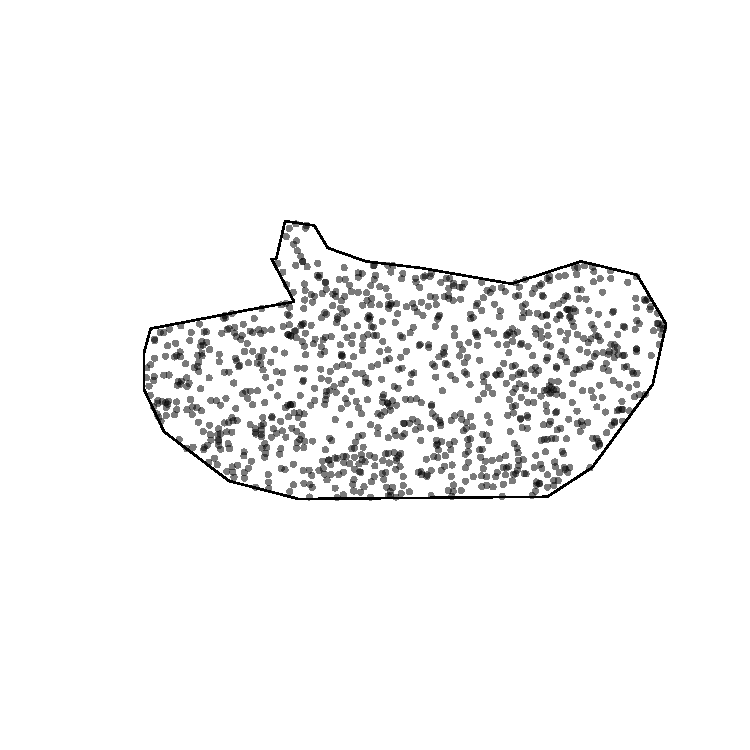
\includegraphics[scale=.4]{poicrows.pdf}
\hspace*{-.5cm} \column{5cm}
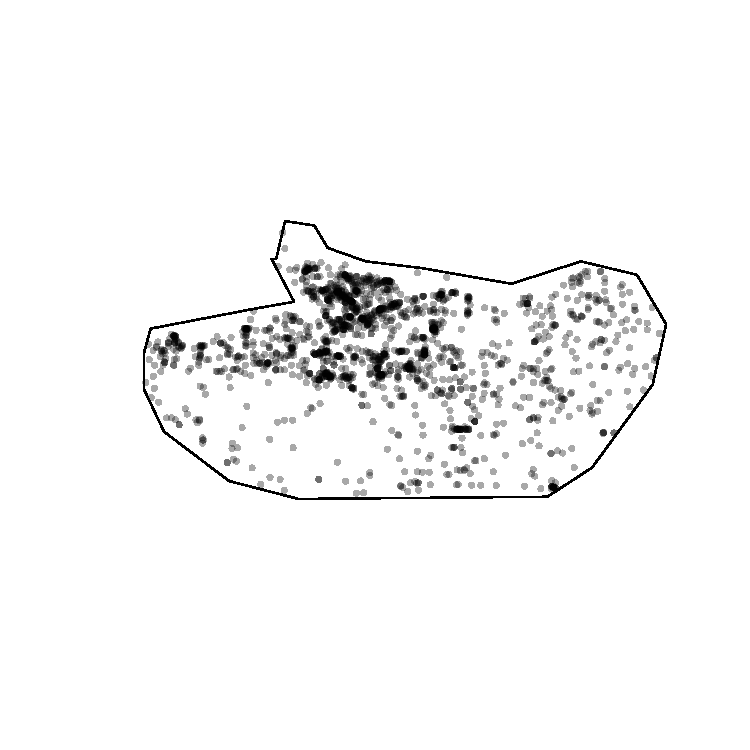
\includegraphics[scale=.4]{crows.pdf}
\column{5cm}

\vspace*{-.3cm}

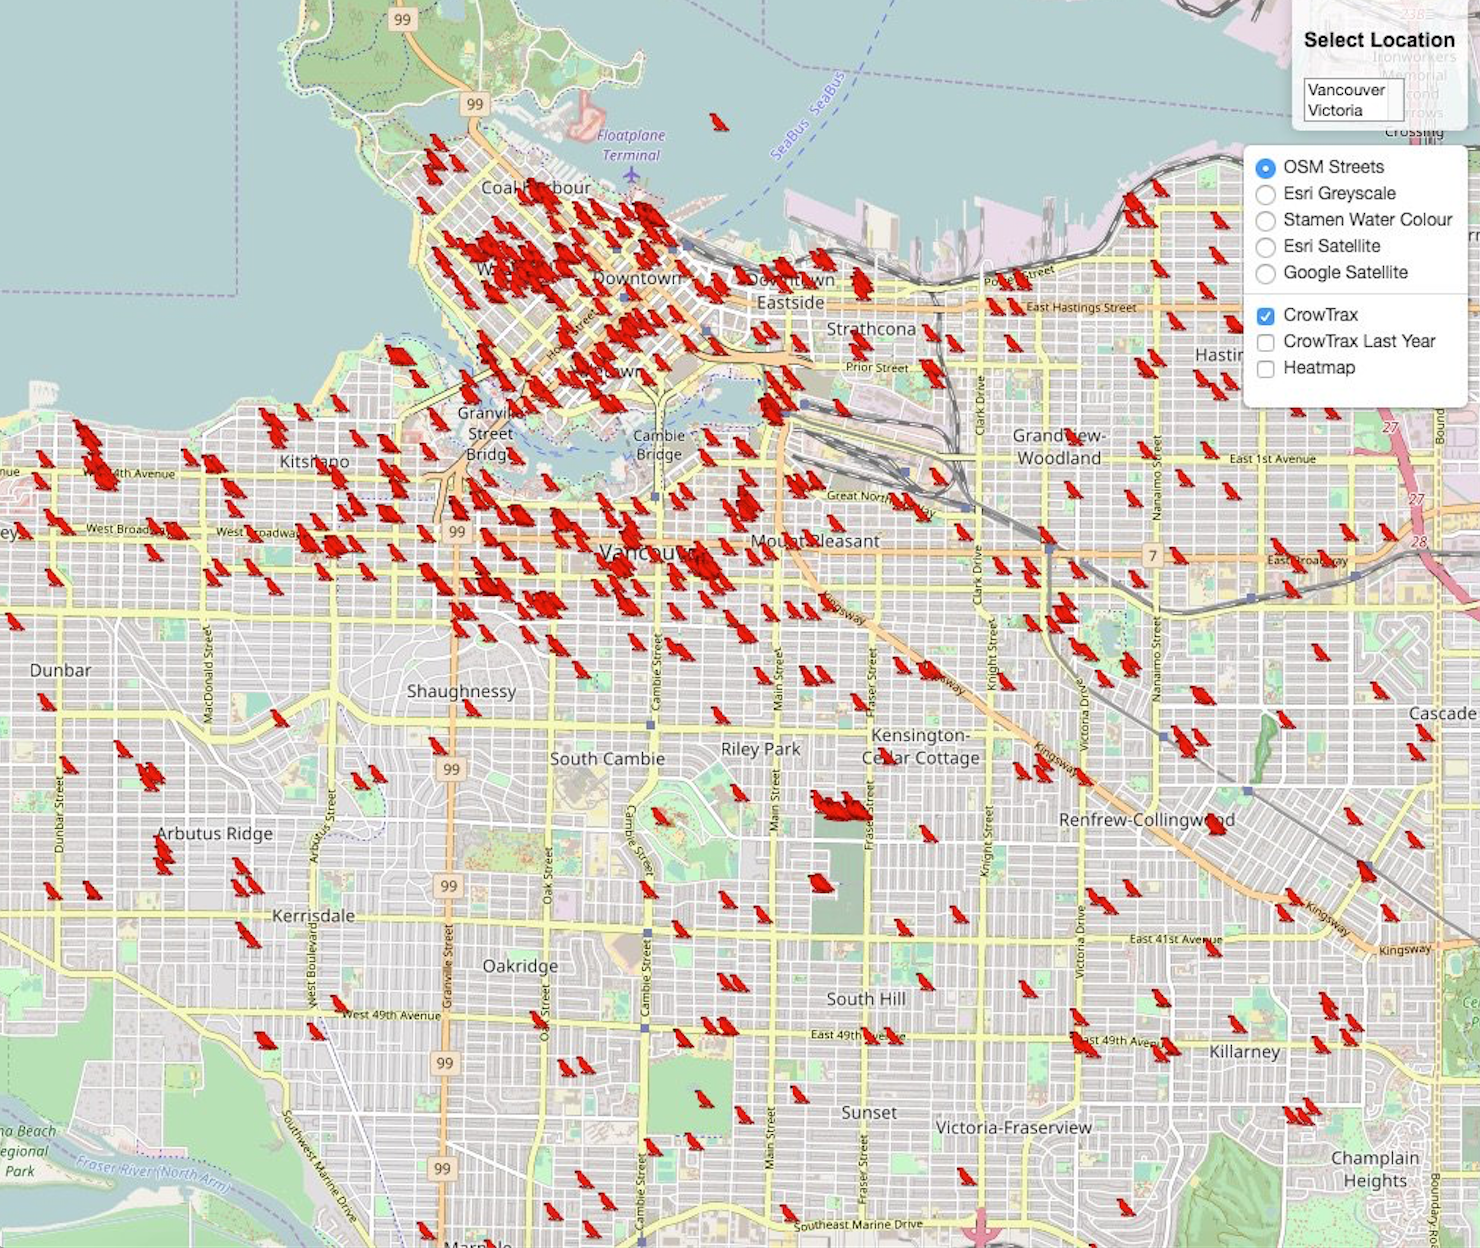
\includegraphics[scale=.1]{crowtrax.png}
	\end{columns}
	
	% \item Exhibit negative or positive dependence

\vspace*{-1.7cm}
\item \dots can exhibit \only<1>{independence, neg. or pos. dependence}\only<2>{\tr{independence, neg. or pos. dependence}}

\vspace*{-.5cm}
\centerline{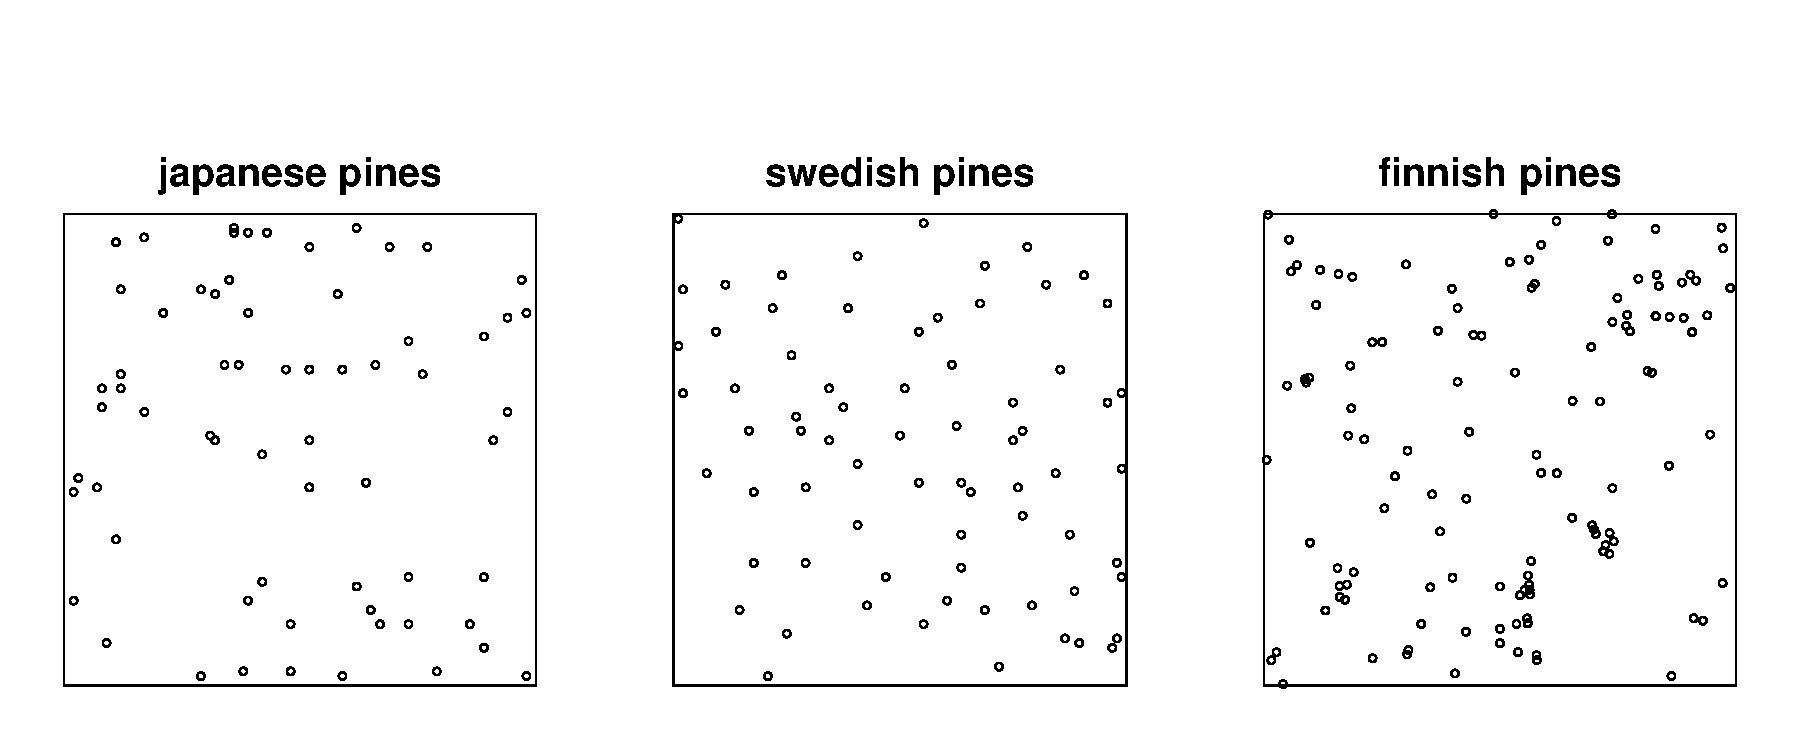
\includegraphics[scale=.27]{trees}}
\end{itemize}
\end{frame}

\begin{frame}{How to characterize or summarize a point process?}

\begin{itemize}
	\item finite-dimensional distributions of counting variables;
	\item void provabilities: $\mathrm P(N(B)=0)$, for any compact set $B$;
	\item via a density (with respect to a Poisson process);
	\item intensity functions: \fbox{\;{$\rho$}\;}, $\rho^{(2)}$, $\rho^{(3)}$,\dots
	\item summary statistics: Ripley's $K$ function, functions $F,G,J,L,\dots$
\end{itemize}


% \hrulefill


\begin{block}{Intensity function: $\rho  : W \to \R^+$}

\vspace*{-.8cm}

\begin{align*}
\rho (u) &\approx \mathrm P \left( \bX \text{ has a point in } B(u,\dd u) \right)\\
\E \sum_{u \in \bX} h(u) & = \int h(u) \rho(u) \dd u, \quad \qquad \text{\small [Campbell Theorem]}
\end{align*}
\end{block}	

% \vspace*{-.5cm}

\underline{Objective:} parametric modeling $\rho$ 


\end{frame}


\begin{frame}{Data: Barro Colorado Island (Hubell et al., 1999, 2005)}

\begin{columns}
\column{6cm}
\begin{itemize}
	\item $W=[0,1000m]\times[0,500m]$
	\item $>300,\!000$ locations of trees
	\item $\approx$ 300 species
	\item $\approx 100$ spatial covariaties observed at fine scale (altitude, nature of soils,\dots)
\end{itemize}
\column{6cm}
	\begin{tabular}{llll}
				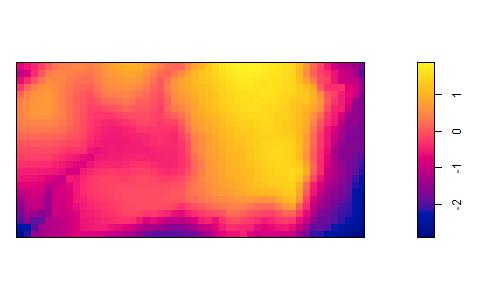
\includegraphics[width=0.23\textwidth]{covar1sim3.jpg} & 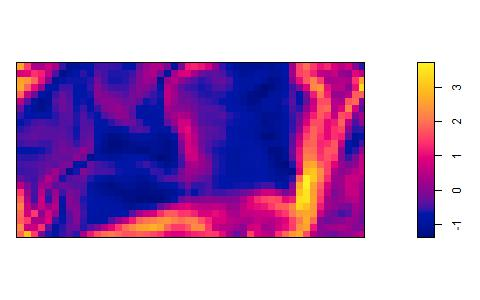
\includegraphics[width=0.23\textwidth]{covar2sim3.jpg} &  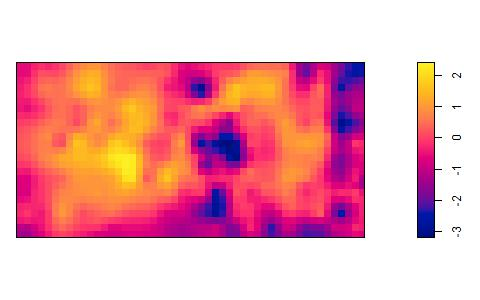
\includegraphics[width=0.23\textwidth]{covar3sim3.jpg} 
			&\dots\\	% & 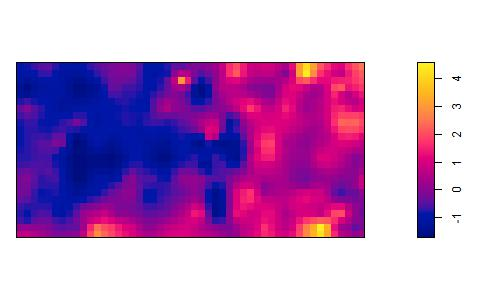
\includegraphics[width=0.23\textwidth]{covar4sim3.jpg} 
				% & 
				% 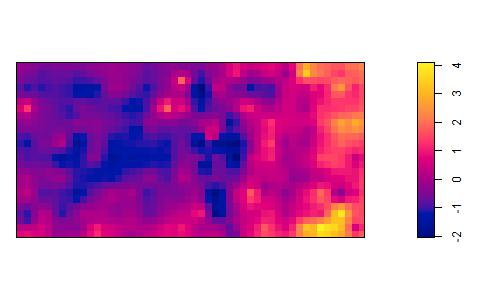
\includegraphics[width=0.23\textwidth]{covar5sim3.jpg}   \\
				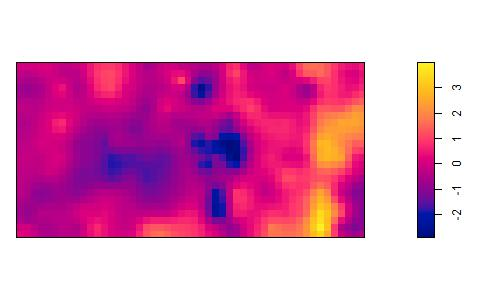
\includegraphics[width=0.23\textwidth]{covar6sim3.jpg} & 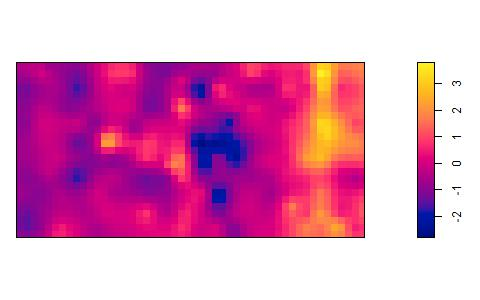
\includegraphics[width=0.23\textwidth]{covar7sim3.jpg} & 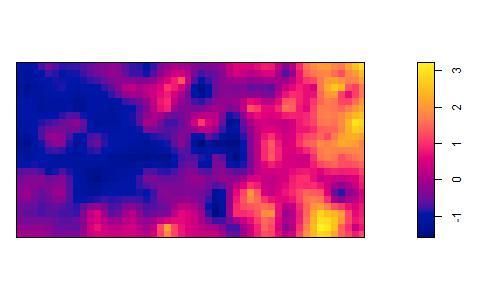
\includegraphics[width=0.23\textwidth]{covar8sim3.jpg}&\dots \\
				% &  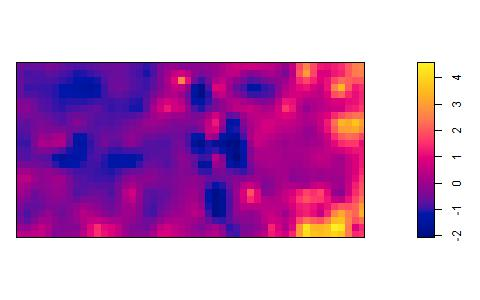
\includegraphics[width=0.23\textwidth]{covar9sim3.jpg} & 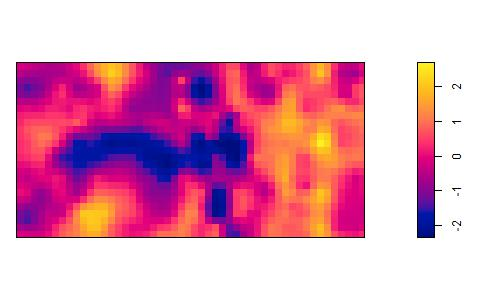
\includegraphics[width=0.23\textwidth]{covar10sim3.jpg} \\ 
				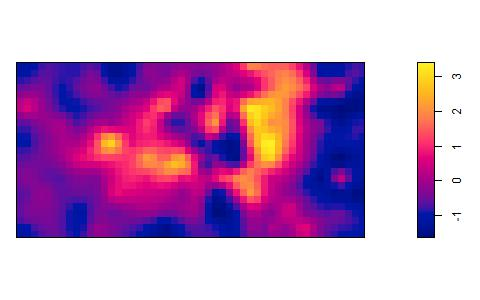
\includegraphics[width=0.23\textwidth]{covar11sim3.jpg} &  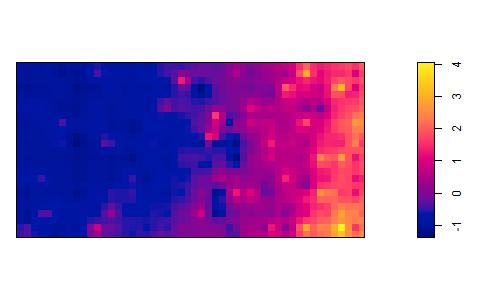
\includegraphics[width=0.23\textwidth]{covar12sim3.jpg} & 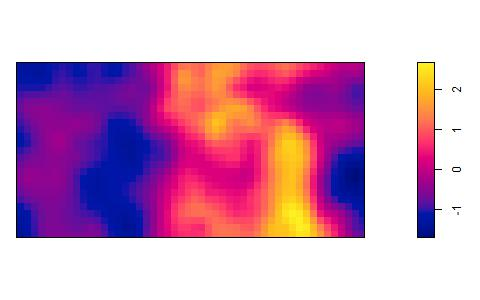
\includegraphics[width=0.23\textwidth]{covar13sim3.jpg} &\dots
				% &  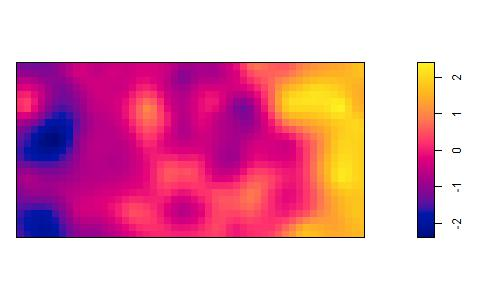
\includegraphics[width=0.23\textwidth]{covar14sim3.jpg} &  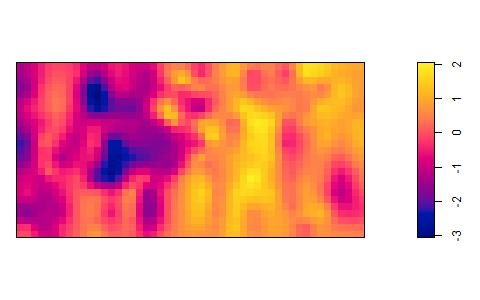
\includegraphics[width=0.23\textwidth]{covar15sim3.jpg} \pause
			\end{tabular}
\end{columns}

\bigskip

\hrulefill

\begin{columns}

\column{5cm}
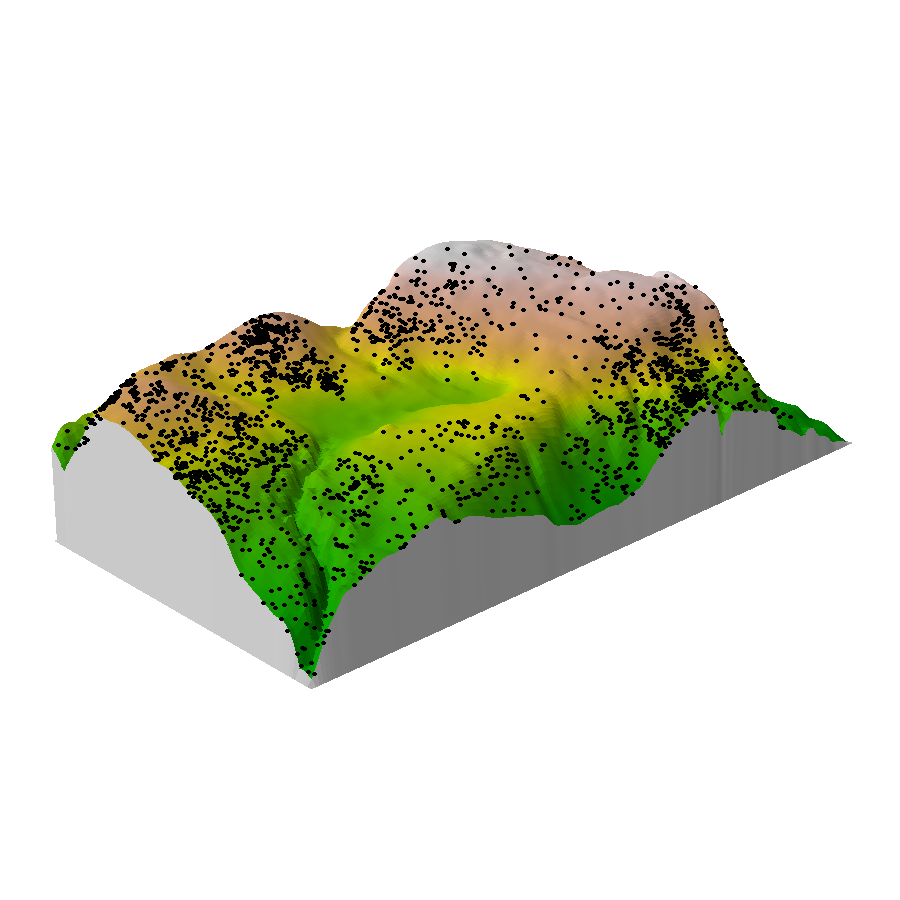
\includegraphics[scale=.3]{bei3d}
\column{7cm}
\underline{Modeling $\rho$}: for one species e.g. 
\[
\log \, \rho(u;\bbeta) = \exp(\bbeta^\top \bz(u)),	
\] 
$\bbeta\in \R^p$, $\bz(u) =(z_1(u),\dots,z_p(u))^\top$

\underline{Problem:} \tr{$p$ large, covariates very correlated.	}
\end{columns}

\end{frame}

\begin{frame}{Estimation of $\bbeta$ when $p$ is moderate (1)}

\centerline{\fbox{ ${\displaystyle 
\hat \bbeta = \mathrm{argmax}_{\bbeta} \,  \ell(\bbeta),  \quad 
\ell(\bbeta) = \sum_{u \in \bX \cap W} \only<2>{\tr{w(u)}}\underbrace{\bbeta^\top \bz(u)}_{\log \rho(u;\bbeta)}  - \int_W \only<2>{\tr{w(u)}}\underbrace{\exp \left( \bbeta^\top \bz(u) \right)}_{\rho(u;\bbeta)} \dd u
}$ 
}}





\bigskip

\begin{itemize}
	\item $\ell$ = log-likelihood if $\bX$ is a Poisson point process; 
	\item but $\ell^{(1)}(\bbeta)$ remains an \textit{unbiased estimating equation} for general point processes. Indeed,
\begin{align*}
	\ell^{(1)}(\bbeta) = \sum_{u\in \bX} \only<2>{\tr{w(u)}}\bz(u) -\int_W \only<2>{\tr{w(u)}}\bz(u) \rho(u;\bbeta) \dd u
\end{align*}
so $\E \ell^{(1)}(\bbeta)=0$ by Campbell Theorem (under the true model). 
\item \only<1>{\phantom{Nothing changes if we add a weight surface $\tr{w(\cdot)}$.}}\only<2>{Nothing changes if we add a weight surface $\tr{w(\cdot)}$!!} 
\end{itemize}
\end{frame}

\begin{frame}{Estimation of $\bbeta$ when $p$ is moderate (2)}



\begin{itemize}
	\item $\hat \bbeta\to \bbeta$ and is asympt. normal ($W=W_n \to \R^d$) for~\dots; 
	\item asympt. cov. matrix  can be optimized in terms of $w(\cdot)$. 
	\item Bermann-Turner approximation:  discretize 
	\[
	\int_W w(u) \rho(u;\bbeta) \dd u \approx \sum_{i=1}^{\tr{n+m}} q_i \, \rho(u_i;\bbeta)	
	\] 
	 $m$: $\#$ dummy points; $n$: $\#$ data points; $q_i$ quadrature weights. Then,  with $y_i=q_i^{-1}\mathbf 1(u_i \in \bX)$
	\begin{align*}
	\!\!\!\!\!\!\!\!\!\!		 	\ell(\beta) &\approx   {\sum_{i=1}^{n+m}}
	q_i \bigg\{ \; y_i  \log \rho(u_i; \bbeta) - \rho(u_i; \bbeta) \;\bigg\}
	\stackrel{\texttt{R}}{=} \underbrace{\texttt{\footnotesize glm(...,family=quasipoisson)}}_{\texttt{spatstat package}}              	
	\end{align*}
	\item BT approx. can be avoided (but $\Var (\hat \bbeta^\prime)> \Var(\hat \bbeta)$)
	\[
		\!\!\!\!\!\!\!\!\!\!\!\!\!\!\!\!\!\!\!\!\! \ell^\prime (\bbeta)=\!\!\!\sum_{u\in \bX\cap W} \!\!\!\log \frac{\rho(u;\bbeta)}{\delta + \rho(u;\bbeta)} - \delta \int_{W}\!\!\log \frac{\rho(u;\bbeta)+\delta}\delta \dd u \approx \dots  \stackrel{R}{=} \texttt{\footnotesize glm(...,binomial)} 
	\]
\end{itemize}

\end{frame}

\begin{frame}{When $p$ is large (even $p=p_n$, $W=W_n\to \R^d$)}

% \begin{minipage}{11cm}
\begin{itemize}
	\item Penalization techniques: $\hat \bbeta = \mathrm{argmax}_{\bbeta} \; Q(\bbeta)$ where\\

	\medskip

	\centerline{\fbox{\qquad \quad ${\displaystyle  Q(\bbeta) = \ell(\bbeta) \; - \; |W_n| \sum_{j=1}^{p_n} \pi_{\lambda_{n,j}} ( |\beta_j|)}$\qquad \quad}}
	
	\medskip

	\begin{list}{$\hookrightarrow$}{}
		\item $\lambda_{n,j}\ge 0$ are regularization parameters
		\item $\pi_\lambda(\cdot):$ penalty function $\underbrace{\text{convex}}_{\|\cdot\|_1,\, \|\cdot\|_2,\dots}$ or $\underbrace{\text{non-convex}}_{\text{SCAD, MC+,\dots}}$ \medskip
		\item Example: adaptive Lasso $\pi_{\lambda_{n,j}} = \lambda_{n,j} |\beta_j|$.
	\end{list} 
	\pause \item Computational point of view: thanks to the BT approximation
	\
	\begin{align*}
		\min \; (-Q(\bbeta)) \; &= \; \min \left(  -\ell(\bbeta) +\text{ penalty }\right)\\
		& = \text{ convex } \; + \; \text{ convex/non-convex} \\
		& \stackrel{\texttt{R}}= \texttt{spatstat} \; + \; \texttt{glmnet / ncvreg}
	\end{align*}
		
\end{itemize}
% \end{minipage}
\end{frame}

\begin{frame}{What can we prove? (well expected results!)}

\vspace*{-.3cm}

\begin{itemize}
	\item $\bbeta=(\bbeta_1^\top,\bbeta_2^\top)^\top$, $\bbeta_1\in \R^s$, $\bbeta_2=0 \in \R^{p_n-s}$.
	\item for the {\it adaptive lasso}: let 
	\[
	a_n= \max_{j=1,\dots,s} \lambda_{n,j}, \qquad b_n = \min_{j={s+1,\dots,p_n}} \lambda_{n,j}.	
	\]
\end{itemize}

\begin{block}{Theorem ($|W_n|\to \infty$, $p_n\to \infty$) {\small [Choiruddin, C., Letué'18]}}
\begin{itemize}
	\item Under some assumptions such that it works \dots
	\item $p_n^3/|W_n|\to 0$, $a_n \sqrt{|W_n|} \to 0$, $b_n \sqrt{|W_n|/p_n^2} \to \infty$.
\end{itemize}
Then, as $n\to \infty$\\ 

\centerline{\fbox{\quad ${\displaystyle
\mathrm P \left( \hat \bbeta_2=0 \right) \to 1 \;\;\text{ and } \;\; \hat \Sigma_n^{-1/2}(\bbeta_1 -\bbeta_1) \stackrel{d}\to N(0,I_s)
}  $\quad }}
\end{block}

\bigskip

\hrulefill

\bigskip

\underline{Technical difficulties}: {\small (compared to standard regr. type problems)}
\begin{itemize}
	\item asymptotic is different.
	\item most importantly: points are {\bf dependent}.
\end{itemize}
\end{frame}


\begin{frame}{For other penalties}

	\vspace*{-.3cm}

	{\footnotesize {\bf Possible?} $\Leftrightarrow$  {$a_n\sqrt{|W_n|} \to 0$}  and {$b_n \sqrt{|W_n|/p_n^2} \to \infty$} }

\vspace*{-.4cm}

	\setlength{\tabcolsep}{5pt}
	\renewcommand{\arraystretch}{1.8}
	\begin{center}
		\begin{threeparttable}
			\begin{tabular}{ l l l l }
				\hline
				\hline
				Method &$a_n$ & $b_n$ & Possible?\\
				\hline
				\hline
				Ridge & $\lambda_n \smash{\displaystyle \max_{j=1,...s} \{|\beta_{0j}|\}}$  & $0$ & \trr{\xmark} \\
				Lasso & $\lambda_n$ & $\lambda_n$ & \trr{\xmark}  \\
				Enet & $\lambda_n \left[(1-\alpha)\smash{\displaystyle \max_{j=1,...s} \{|\beta_{0j}|\}}+\alpha \right]$ & $\lambda_n \alpha$ & \trr{\xmark}   \\
				ALasso & $\smash{\displaystyle \max_{j=1,...s} \{\lambda_{n,j}\}}$ & $\smash{\displaystyle \inf_{j=s+1,...p} \{\lambda_{n,j}\}}$ & \tv{\cmark} \\ 
				Aenet & $ \smash{\displaystyle \max_{j=1,...s}\{ \lambda_{n,j}\big((1-\alpha) |\beta_{0j}|+\alpha\big) \}}$  & $\alpha \smash{\displaystyle \inf_{j=s+1,...p}\{\lambda_{n,j} \}}$ & \tv{\cmark}  \\ 
				SCAD & $0 \tnote{*}$ & $\lambda_n \tnote{*}$ & \tv{\cmark}\\ 
				MC+ & $0  \tnote{*}$ & $\lambda_n - \frac {K} {\gamma \sqrt{|D_n|}}  \tnote{*}$ & \tv{\cmark} \\ 
				\hline
			\end{tabular}
			{\footnotesize\begin{tablenotes}
				\item[*] if $\lambda_n \to 0$ and  $\lambda_n\sqrt{|W_n|/p_n^2} \to \infty$.
			\end{tablenotes}}
		\end{threeparttable}
	\end{center}
\end{frame}

\begin{frame}{Short simulation}

\vspace*{-.2cm}

\begin{itemize}
	\item $W=[0,1000]\times [0,500]$; $\bX$: Thomas process (generates clustered patterns); $m=5,\!000$ replications.
	\item $\lambda_{n,j}= \lambda / |\tilde \beta_j|$, $\tilde \beta$ is the non-regularized estimator (or ridge); $\lambda$ is chosen using {\sc bic}-type criterion (\textsc{cv} is dangerous in this setting).
	
\end{itemize}

\vspace*{-.5cm}

\begin{columns}
\column{8cm}
\begin{itemize}
	\item $\bz(u) = (\underbrace{z_1(u),z_2(u)}_{\text{true BCI cov.}},\underbrace{z_3(u),\dots,z_{100}(u)}_{\text{noisy correlated cov.}})^\top$
	\item the $z_i$'s are then centered and reduced; $\beta_1=2$, $\beta_2=.75$.
\end{itemize}
\column{4cm}
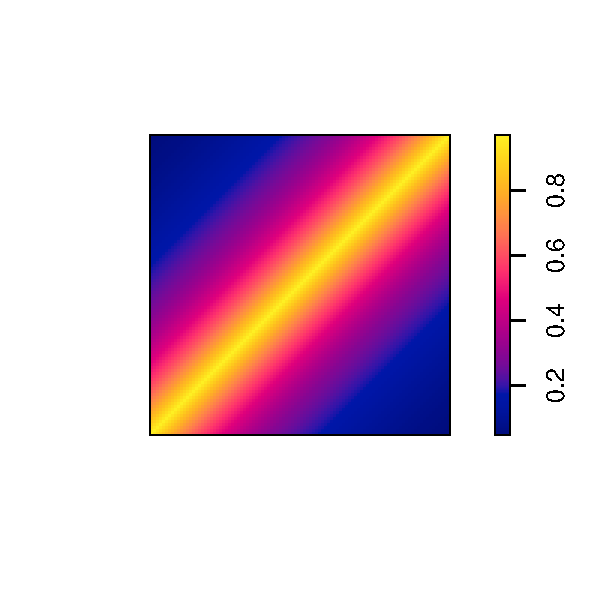
\includegraphics[scale=.3]{corrX}
\end{columns}


\begin{columns}
\column{6cm}	
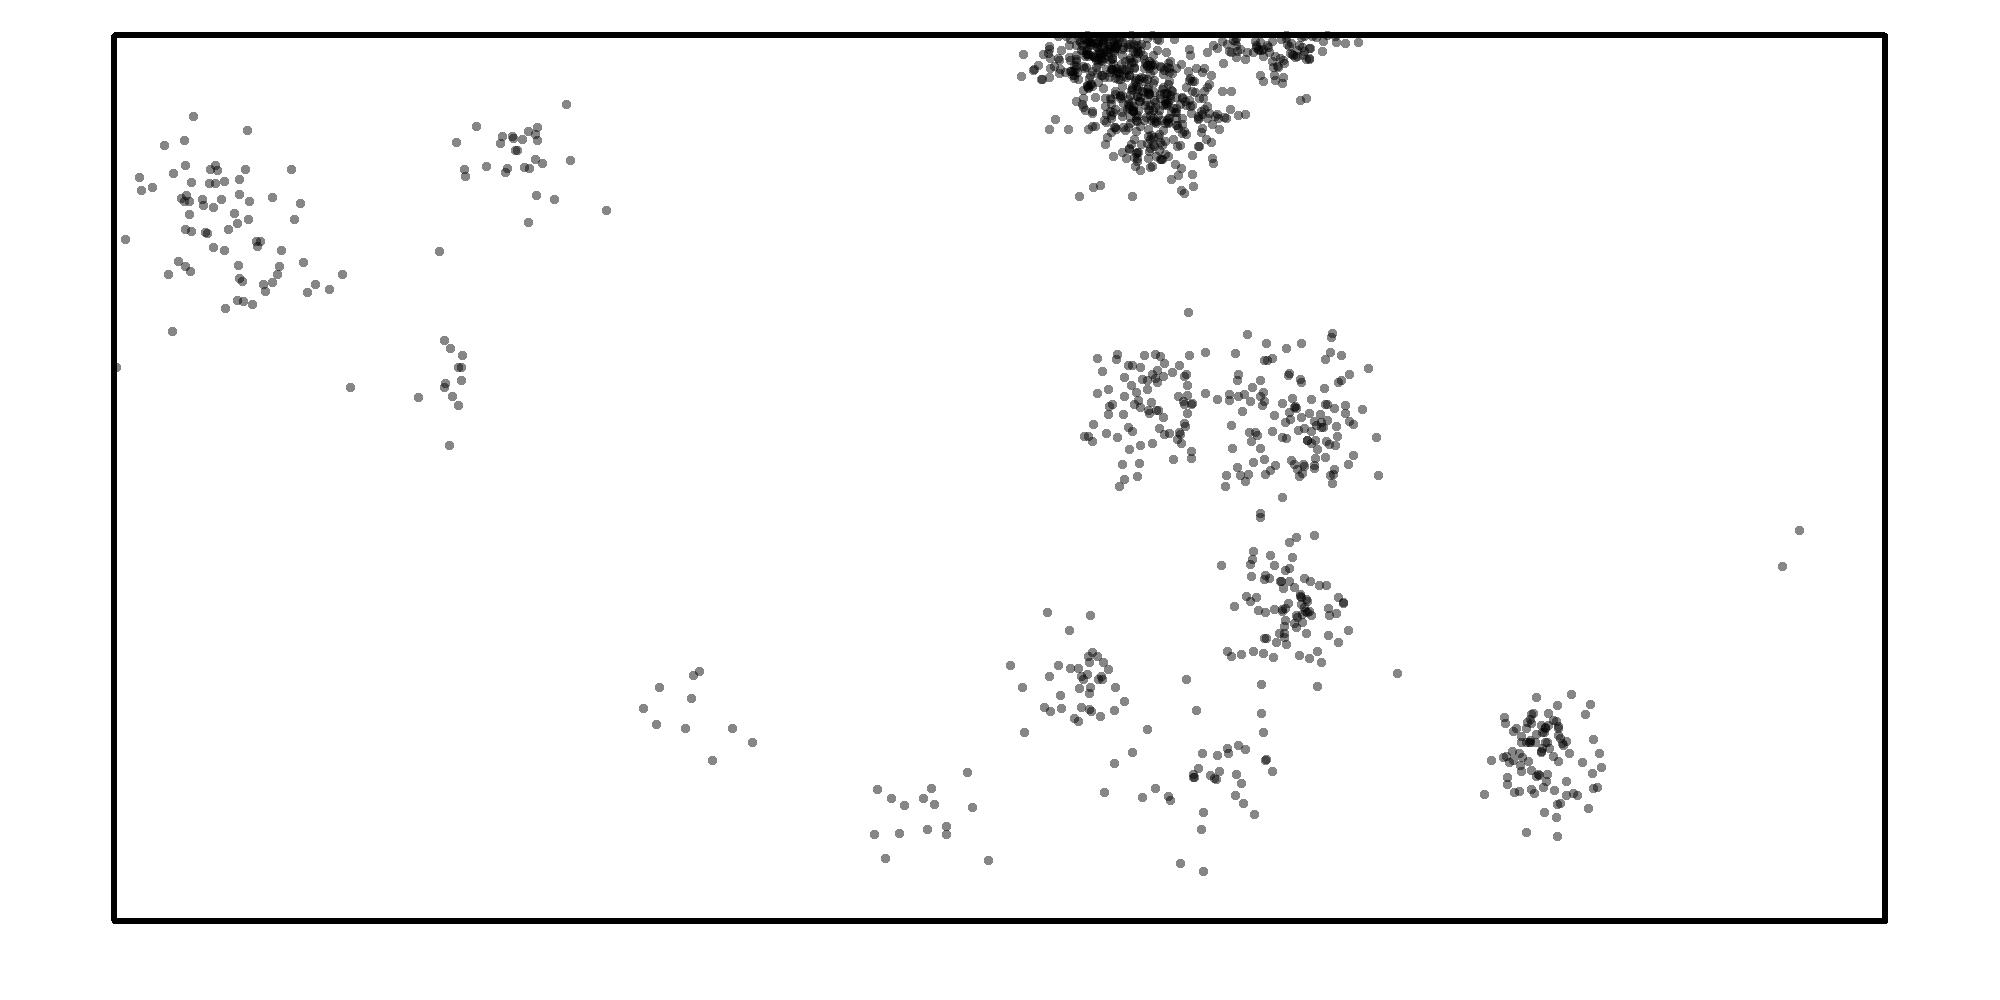
\includegraphics[scale=.07]{thomas4.jpg}
\column{6cm}
{\small 
\hspace*{-1cm}
\begin{tabular}{llll}
\hline 
 &\multicolumn{3}{c}{1600 points in average}\\
&&&\\
& FPR (\%) & FNR (\%)& RMSE  \\
\hline
Lasso &97 & 23  & 0.73\\
A. Lasso &95&3& 0.63\\
SCAD&96 & 7& 0.65\\
\hline
\end{tabular}
}
\end{columns}



\end{frame}

\begin{frame}{Additional remarks and perspectives}

\vspace*{-.3cm}

\begin{itemize}
	\item Applied to the \texttt{bei} dataset - selection of 8 (relevant) covariates (among 93);  higher AUC.
	\item current work: compare AL with {\bf Dantzig type selector}
\[
	\text{Minimize }\sum_{j} \lambda_{n,j} |\beta_j| \quad\text{ subject to } \quad\| \ell^{(1)}(\bbeta)\| \le \lambda_{n,j}
 \]
 \item  300 species of trees?  {\bf high-dimensional multivariate LGCP} (much more challenging): for $i=1,\dots,300$
\[
	\Lambda_i(u) = \rho(u;\bbeta_i) \exp Z_i(u) \quad Z_i(u) =  \sum_{l=1}^q \alpha_{il} E_{l}(u) + U_i(u)
\]
\begin{list}{$\hookrightarrow$}{}
	\item $E_l, U_i$ are indep. stationary Gaussian random fields; 
	\item typically approx. 10,000 interaction parameters
\end{list}

\end{itemize}

\hrulefill

{\scriptsize Choiruddin , {\bf C.}, Letué. {\it Convex and non-convex regularization methods for spatial point processes intensity estimation}, EJS, 12(1):1210–1255, 2018.}
\end{frame}

\end{document}




